\documentclass[]{article}
\usepackage{lmodern}
\usepackage{amssymb,amsmath}
\usepackage{ifxetex,ifluatex}
\usepackage{fixltx2e} % provides \textsubscript
\ifnum 0\ifxetex 1\fi\ifluatex 1\fi=0 % if pdftex
  \usepackage[T1]{fontenc}
  \usepackage[utf8]{inputenc}
\else % if luatex or xelatex
  \ifxetex
    \usepackage{mathspec}
  \else
    \usepackage{fontspec}
  \fi
  \defaultfontfeatures{Ligatures=TeX,Scale=MatchLowercase}
\fi
% use upquote if available, for straight quotes in verbatim environments
\IfFileExists{upquote.sty}{\usepackage{upquote}}{}
% use microtype if available
\IfFileExists{microtype.sty}{%
\usepackage{microtype}
\UseMicrotypeSet[protrusion]{basicmath} % disable protrusion for tt fonts
}{}
\usepackage[margin=1in]{geometry}
\usepackage{hyperref}
\hypersetup{unicode=true,
            pdfborder={0 0 0},
            breaklinks=true}
\urlstyle{same}  % don't use monospace font for urls
\usepackage{graphicx,grffile}
\makeatletter
\def\maxwidth{\ifdim\Gin@nat@width>\linewidth\linewidth\else\Gin@nat@width\fi}
\def\maxheight{\ifdim\Gin@nat@height>\textheight\textheight\else\Gin@nat@height\fi}
\makeatother
% Scale images if necessary, so that they will not overflow the page
% margins by default, and it is still possible to overwrite the defaults
% using explicit options in \includegraphics[width, height, ...]{}
\setkeys{Gin}{width=\maxwidth,height=\maxheight,keepaspectratio}
\IfFileExists{parskip.sty}{%
\usepackage{parskip}
}{% else
\setlength{\parindent}{0pt}
\setlength{\parskip}{6pt plus 2pt minus 1pt}
}
\setlength{\emergencystretch}{3em}  % prevent overfull lines
\providecommand{\tightlist}{%
  \setlength{\itemsep}{0pt}\setlength{\parskip}{0pt}}
\setcounter{secnumdepth}{0}
% Redefines (sub)paragraphs to behave more like sections
\ifx\paragraph\undefined\else
\let\oldparagraph\paragraph
\renewcommand{\paragraph}[1]{\oldparagraph{#1}\mbox{}}
\fi
\ifx\subparagraph\undefined\else
\let\oldsubparagraph\subparagraph
\renewcommand{\subparagraph}[1]{\oldsubparagraph{#1}\mbox{}}
\fi

%%% Use protect on footnotes to avoid problems with footnotes in titles
\let\rmarkdownfootnote\footnote%
\def\footnote{\protect\rmarkdownfootnote}

%%% Change title format to be more compact
\usepackage{titling}

% Create subtitle command for use in maketitle
\newcommand{\subtitle}[1]{
  \posttitle{
    \begin{center}\large#1\end{center}
    }
}

\setlength{\droptitle}{-2em}

  \title{}
    \pretitle{\vspace{\droptitle}}
  \posttitle{}
    \author{}
    \preauthor{}\postauthor{}
    \date{}
    \predate{}\postdate{}
  

\begin{document}

\chapter{Methods}\label{ch:methods}

\section{Making social care data available for linkage}\label{sec:linkage}

Describe method of matching SCS to Population Spine

\section{Creating a linked health and social care dataset}\label{sec:make-dataset}

\FloatBarrier

\subsection{Setting and cohort}\label{subsec:setting-cohort}

Setting?? Scotland 5 mill, 32 LA, 14 HB etc..

The study cohort included all individuals in Scotland born before 31st
March 1951 and alive during the study period 1st April 2011 to 31st
March 2016. This identified all those over the age of 65 (and those
turning 65 during the study period). Data for the cohort was extracted
from the research population spine held by NRS with CHI numbers allowing
linkage to other health datasets.

\begin{landscape}
\begin{figure}
  \centering
    \caption{Data linkage diagram}
    \includegraphics{data/produced_data/linkage-diagram/linkage-diagram.pdf}
    \label{fig:methods-linkage}
\end{figure}
\end{landscape}

As figure \ref{fig:methods-linkage} shows linkage keys from the
extracted cohort were sent by an eDRIS coordinator to various health and
social care data sources for extraction of information relating to any
of these indivudals in the target data source. Specific variables
requested, the time period they were requested over, and cleaning and
wrangling of these data sources is described in the following section.

\textbf{Figure needs tidied up and should show datasets in same order as
follwoing subsections}

The aim of cleaning and wrangling was to create one row of data for each
indivudal for each financial year (1st April - 31st March) of the study
period. This format is based on the principals of tidy data
{[}@RN553{]}. Financial years were chosen as the time period of interest
because the social care survey reports home care usage in a census week
which is usually at the end of March. As each raw data file provided was
in differing formats, this required differing approaches and relied
heavily on data manipulation software packages \texttt{tidyr} v0.7.2
{[}@RN524{]}, \texttt{dplyr} v0.7.4 {[}@RN283{]}, \texttt{lubridate}
v1.6.0 {[}@RN522{]}, \texttt{stringr} v1.2.0 {[}@RN554{]}, and
\texttt{forcats} v0.2.0 {[}@RN521{]} in the R language and environment
for statistical computing version 3.4.0 {[}@RN295{]} via the Integrated
Development Environment RStudio v1.0.143 {[}@RN498{]}.

\FloatBarrier

\subsection{Demographic, geographic, and deaths information}\label{subsubsec:nrs-summs}

Which years of data

Which Local Authority? Which SIMD data

\begin{table}[h]
\centering
\caption{Demographic file data}
\label{tab:demos}
\resizebox{\textwidth}{!}{%
\begin{tabular}{@{}lll@{}}
\toprule
Number of rows & Number of individuals & Variables \\ \midrule
1,348,310 & 1,134,445 & \begin{tabular}[c]{@{}l@{}}Index, year/month of birth, year/month of death\\ Sex, Address start date, Address end date, Care home flag,\\ Previous Local Authority, Current Local Authority, \\ Current Health Board, SIMD decile\end{tabular} \\ \bottomrule
\end{tabular}%
}
\end{table}

Demographic information for all eligible indiviudals identified from the
population spine was extracted by the Public Health and Intelligence:
Strategic Business Unit at NSS. This was joined with a flag variable
indicating if an individual was resident in a care home (from
prescribing data) in a single file which was made available in the
national safe haven. SIMD decile was assigned as per the most recent
version of the area-based measure (2016). The number of observations,
individuals, and the differing variables in this raw demographic file
are shown in table \ref{tab:demos}.

As the table indicates some individuals had more than one row of
information indicating multiple addresses during the study period (and
thus potential multiple values for local, authority, health board, care
home flag, and SIMD decile). Financial year time intervals were created
for each financial year using the \texttt{lubridate} software package
{[}@RN522{]}. Dummy variables were then created indicating the age,
local authority of residence, health board of residence, and simd decile
during each financial year (with null values where not applicable). The
variables were then gathered to long format in order to reshape the data
to include one row of data per individual per financial year. This
resulted in a dataframe of 7,775,410 observations pertaining to
1,134,445 individuals.

\FloatBarrier

\subsection{Social Care Survey}\label{subsubsec:scs-summs}

Which years of data

Which variables were used and how summarised and cleaned (i.e.~telecare
as categorical etc.)

with reference to chapter \ref{ch:renfrew} and measure of hours of
social care

\subsection{Prescribing Information Service}\label{subsubsec:pis-summs}

data from 2010 onwards (to allow calc of MM in year previous to SC)

describe variables

How PIS data was summarised and measures chosen

\subsection{Unscheduled care measures}\label{subsubsec:usc-summs}

Which years of data (remember OOH from 2014 onwards only)

How was usc data wrangled? Which summary measures were chosen?

\subsection{Joining sources together}\label{subsubsec:join-data}

\section{Statistical methods}\label{sec:methods-stats}

\subsection{Descriptive statistics}\label{descr}

\subsection{Research question 1}\label{stats-rq1}

\subsection{Research question 2}\label{stats-rq2}


\end{document}
